\documentclass[a4paper,12pt,oneside,openany]{jsbook}
%%%%%%%%%%%%%%%%%%%%%%%%%%%%%%%%%%%%%%%%%%%%%%%%%%%%%%

\usepackage{subfigure}
\usepackage{amsmath,amssymb,latexsym,bm}
\usepackage[dvipdfmx]{graphicx}
\usepackage[dvipdfmx]{color}
\usepackage{appendix}
\usepackage{titlesec}
\usepackage{amsthm}
% \usepackage{algorithmic}
\usepackage{algorithm}
\usepackage{algpseudocode}

\usepackage{amsfonts} % 数学記号用
\renewcommand{\proofname}{\textbf{証明}}



\newtheorem{thm}{定理}[chapter]
\newtheorem{deff}{定義}[chapter]
\newtheorem{sub}{補題}[chapter]
\newtheorem{rem}{注意}[chapter]
\newtheorem{ex}{例}[chapter]
\newcommand{\argmax}{\mathop{\rm arg~max}\limits}


\makeindex
%%% 余白・文字数調整(左37mm, 右18mm, 上下共30mm, 文字数約40字/行, 行数約32行)
\setlength{\textwidth}{150truemm}      % テキスト幅: 210-(30+30)=150mm
%\setlength{\fullwidth}{\textwidth}     % ページ全体の幅
\setlength{\oddsidemargin}{30truemm}   % 左余白
\addtolength{\oddsidemargin}{-1truein} % 左位置デフォルトから-1inch
\setlength{\topmargin}{30truemm}       % 上余白
\setlength{\textheight}{210truemm}     % テキスト高さ: 297-(30+30)=237mm
\addtolength{\topmargin}{-1truein}     % 上位置デフォルトから-1inch
\makeatother
%
%% <local definitions/>


% 本文の行数と桁数を指定出来るように
\def\linesparpage#1{\baselineskip=\textheight
   \divide\baselineskip by #1}
\def\kcharparline#1{%
   \ifx\xkanjiskip\undefined%
   % NTT jTeX用
   \jintercharskip 0mm plus 0.2mm minus 0.2mm
   \else
   % ASCII pTex用
   \xkanjiskip 0mm plus 0.2mm minus 0.2mm
   \fi
   \settowidth{\textwidth}{あ}%
   \multiply\textwidth by #1}
%
%
{\large
\begin{document}
\kcharparline{40} % 一行を40字に
%%% タイトル設定

\begin{titlepage}
\begin{center}
	{\Large 卒業論文\\}
	\vspace{ 5mm }
	\baselineskip 35pt plus 1pt minus 1pt
	{\bf {\huge マルコフパラメータ推定における \\物理制約下での入力設計}}
	
	\vspace{ 30mm }
	{\LARGE 片岡 慎治 \\}
	
	\vspace{ 10mm }
	{\large 大阪大学工学部 応用自然科学科\\}
	{\large 応用物理学科目\\}
	
	\vspace{ 10mm }
	{\large 指導教員\\}
	{\large 和田 孝之 准教授 \\}
	
	\vspace{ 5mm }
	\begin{figure}[h]
	\centering
	
\includegraphics[width=20mm]{osaka_logo.pdf}\\
	\end{figure}
	\vspace{ 5mm }
	{\large 令和 7年 2月 6日}
\end{center}
\end{titlepage}
\thispagestyle{empty}

%%%%%%%%%%%%%%%%%%%%%%%%%%%%%%%%%%%%%

\frontmatter

\tableofcontents

\mainmatter
% %
% \include{chap1}
\chapter{序論}

\section{背景}
システム同定とは,入出力のデータからシステムのダイナミクスを推定することであり,制御システムの効率的かつ高精度な設計,システムの動作予測,故障診断などにおいて重要な役割を果たす\cite{SSSS, SITF}.
特に線形システムは,その扱いやすさから製造業におけるロボットの制御や自動車産業における安定性制御,経済学では市場予測や価格変動モデルなど幅広い分野で近似モデルとして採用されている.
これまでシステム同定の研究では,収集された入出力データのサンプル数を無限に仮定した漸近的な解析が主流であり,入出力のデータ数が無限に増加する場合における性能保証が中心的なテーマだった.
しかし,現実においては利用可能なデータが有限である場合が一般的であり,漸近的な結果に基づく設計では実用上の精度が保証されないことがある.また,故障確率や過渡現象などの概念を解析するのに適しているといった理由で,非漸近的な解析が注目されるようになり,有限のデータにおける特性を解析する研究が行われてきた.

近年の研究動向として,高次元統計\cite{HDPA, HDSA}や機械学習理論\cite{TEOS}の発展に伴い,これらのツールを活用することで非漸近的な解析における理論的基盤がさらに強化された.特に,線形システムにおける有限の入出力データを用いた解析に関する理論が整備され,システムパラメータを所定の精度レベルで同定するために必要なデータ数の下限を導出するための情報理論的議論もされている.これにより,システムの学習効率を定性的に評価できるようになった\cite{SLTF}.

その中でも,線形時不変システムの同定は,構造がシンプルでありながら広範な応用が可能であるため,従来から盛んに研究されてきた.
特に入出力データから得られるシステム行列の最小二乗推定値について,誤差境界やサンプル複雑性が議論されてきた.
線形システムにおいて最も基本的なケースである,入力を印加しない完全観測システムについて,システム行列の最小二乗推定値に関する有限時間での推定誤差の上界や任意の精度を保証するために必要なデータ数の下界を導出している\cite{FTIIU, FTIOL}.
また,入力を印加するシステムについてシステム行列の誤差を制御設計に適用し最適二次レギュレータを用いて安定化制御を可能にする推定誤差とサンプル複雑性について議論されている\cite{OTSCO}.

入出力データからシステム同定をする手法の一つとして,パルス伝達関数の係数であるマルコフパラメータを推定する手法がある.
システムが安定な場合についてひとつの軌道の入出力データから,安定性を要求しない場合について複数の独立した軌道の入出力データから,それぞれマルコフパラメータ行列の最小二乗推定値の推定誤差の上界を導出している\cite{RHKB, NAIOL}.


\section{目的}
システムの入出力関係を示すマルコフパラメータを推定することは,直接的にシステムの入出力の関係を表すことができる点から,重要である.従来の手法では,入力が正規分布に従って生成されるというケースが一般的であり,入力信号に制約を設けず,理想的に設計可能であることを前提としている.
一方,現実の物理的なシステムでは,理想的な乱数に従う入力信号を生成することが困難な場合や,アクチュエータの物理的制約によって入力の大きさに上限が課される場合,電池駆動のシステムにおける電流の制限など,実際の応用環境では様々な制約が課されることが多い.そのため入力に制約がある場合でも適用可能な理論的保証が求められる.
このため本研究では,物理的な制約を考慮し,入力の大きさに上界がある条件下において有限の入出力データから高精度な推定値を得る入力設計手法を確立し,理論的な保証を与えることを目的とする.

\section{構成}
本論文の構成は以下の通りである.
まず,第2章では,マルコフパラメータおよび対象とするシステムの設定など,本論文で用いる数学的概念の定義を行い,マルコフパラメータの最小二乗推定の手順について述べる. 
また,先行研究の入力が正規分布に従い生成される場合のマルコフパラメータの推定精度について紹介する.
第3章では入力の大きさに上限がある場合にも適用可能な,本論文で提案する入力設計アルゴリズムを紹介し,数値実験から最良の入力を得ることのできる確率分布について検討している.
また,入力が決定した場合のマルコフパラメータ行列の推定誤差のスペクトルノルムについての上界を導出している.
最後に第4章で結論を述べる.



\chapter{入力に制約がない場合のマルコフパラメータ推定}
\section{問題設定}
以下の離散時間線形時不変システム
\begin{align}
    \label{state1}
    x_{t+1} &= Ax_t + Bu_t + w_t \\
    \label{output1}
    y_t &= Cx_t + Du_t + z_t
\end{align}
を考える.ただし,
$x_t \in \mathbb{R}^n,u_t \in \mathbb{R}^p,y_t \in \mathbb{R}^m$はそれぞれ時刻$t$におけるシステムの状態,入力,出力を表す.また,$w_t \in \mathbb{R}^n,z_t \in \mathbb{R}^m$はプロセスノイズおよび観測ノイズを表し,$w_t \sim \mathcal{N}(0, \sigma_w^2I), z_t \sim \mathcal{N}(0, \sigma_z^2I)$である.
初期状態$x_1 = 0$であり,$\rho(A) \leq \eta <1$を仮定する.ここで,$\rho(\cdot)$は行列の最大固有値の絶対値を表す.

本章では,未知の行列$A,B,C,D$を推定することを目的とする.

\section{マルコフパラメータについて}
システム\eqref{state1}, \eqref{output1}において,入出力関係は
\begin{equation*}
    y_t = Du_t+ \sum_{i = 1}^{t-1}CA^{i-1}Bu_{t-i} + \sum_{i = 1}^{t-1}CA^{i-1}w_{t-i}
\end{equation*}
と表される.このときの入力の係数行列である$D, CB, CAB, CA^2B, \ldots$をシステムのマルコフパラメータと呼ぶ.



また,システムの最初の$T$個のマルコフパラメータを並べた行列を
\begin{equation}
    G = 
    \begin{bmatrix}
        D & CB & CAB & \ldots & CA^{T-2}B
    \end{bmatrix}
    \in \mathbb{R}^{m \times pT}
\end{equation}
と定義し,この$G$の推定を目的とする.
次の節では,この$G$の最小二乗推定の手順について説明する.

\section{マルコフパラメータの最小二乗推定の手順}

まず,推定手順を説明するために,データ収集の方法について説明する.
今回,システムの入出力データを時間長$\bar{N}$まで取得する。このとき得られるデータセットは  
\begin{equation*}
    \{(y_t, u_t):t = 1, 2, \ldots,  \bar{N} \}
\end{equation*}
である.
この与えられたデータセットから長さ$T$のセットを$N$個生成する.
$\bar{N} = N + T - 1$である.
ある時刻$t$において入力,ノイズを時間長$T$分並べたものを
\begin{align}
    \bar{u}_t &= 
    \begin{bmatrix}
        u_t^* & u_{t-1}^* & \ldots & u_{t-T+1}^*
    \end{bmatrix}^*
    \in \mathbb{R}^{pT}
    \\
    \bar{w}_t &= 
    \begin{bmatrix}
        w_t^* & w_{t-1}^* & \ldots & w_{t-T+1}^*
    \end{bmatrix}^*
    \in \mathbb{R}^{nT}
\end{align}
と表記する.
$y_t$を$t-T+1$まで再帰的に展開すると,出力$y_t$と$\bar{u}_t$,$G$の関係は
\begin{align}
    y_t &= Cx_t + Du_t + z_t \notag \\
        &= C(Ax_{t-1} + Bu_{t-1} + w_{t-1}) + Du_t + z_t \notag  \\
        \label{u_y}
        &= G\bar{u}_t + F\bar{w}_t + z_t + e_t 
\end{align}
となる.ここで,
$F = 
\begin{bmatrix}
    0 & C & CA & \ldots & CA^{T-2}
\end{bmatrix}\in \mathbb{R}^{m \times nT}$
であり,
$e_t = CA^{T-1}x_{t-T+1}$
は,時刻$t-T+1$におけるシステムの状態の影響による誤差に相当する.
この関係を用いて,$N$個の$(\bar{u}_t, y_t)_{t = T}^{\bar{N}}$を入出力データとして扱う.

上の\eqref{u_y}式右辺の2項目以降をノイズとして最小二乗法を適用すると$G$の最小二乗推定値は,
\begin{equation}
\label{least_square}
    \hat{G} = \underset{X \in \mathbb{R}^{m \times pT}}{\text{arg min}} \sum_{t = T}^{\bar{N}} \| y_t - X\bar{u}_t \|^2 
\end{equation}
と表せる.
ただし,$\| \cdot \|$はスペクトルノルムを表す.
また,
\begin{align}
    Y &=
    \begin{bmatrix}
        y_T & y_{T+1} & \ldots & y_{\bar{N}}
    \end{bmatrix}^*\in \mathbb{R}^{N \times m}  \\
    \label{U}
    U &=
    \begin{bmatrix}
        \bar{u}_T & \bar{u}_{T+1} & \ldots & \bar{u}_{\bar{N}}
    \end{bmatrix}^*\in \mathbb{R}^{N \times pT}
\end{align}
と定義すると,\eqref{least_square}式より,
\begin{equation}
    \hat{G} = \underset{X \in \mathbb{R}^{m \times pT}}{\text{min}}  \| Y - UX^* \|_F^2
\end{equation}
となる.なお,$\|\cdot\|_F$はフロベニウスノルムを表す.
最小二乗解である$\hat{G}$は,
\begin{equation}
    \label{hatG}
    \hat{G} = (U^{\dag}Y)^*
\end{equation}
と与えられる.
ここで,$U^{\dag} = (U^*U)^{-1}U^*$は左疑似逆行列である.また,
\begin{align}
    \label{W_norm}
    W &=
    \begin{bmatrix}
        \bar{w}_T & \bar{w}_{T+1} & \ldots & \bar{w}_{\bar{N}}
    \end{bmatrix}^*\in \mathbb{R}^{N \times pT}\\
    \label{E}
    E &=
    \begin{bmatrix}
        e_T & e_{T+1} & \ldots & e_{\bar{N}}
    \end{bmatrix}^*\in \mathbb{R}^{N \times m}\\
    Z &=
    \begin{bmatrix}
        z_T & z_{T+1} & \ldots & z_{\bar{N}}
    \end{bmatrix}^*\in \mathbb{R}^{N \times m}
\end{align}
と定義すると,システムの入出力関係を以下のように記述することができる.
\begin{equation}
    Y = UG^*+E + Z + WF^*
\end{equation}
$G$について解くと$G^* = U^{\dag}(Y - E - Z - WF^*) $となるため,
(\ref{hatG})式より最小二乗推定値と真値の誤差は,
\begin{equation}
    \label{error}
    (\hat{G} - G)^* = (U^*U)^{-1}U^*(E + Z +WF^*) 
\end{equation}
となる.

\section{先行研究における推定精度}
先行研究では入力を$\mathcal{N}(0, \sigma_u^2I_p)$に従い生成した場合について$G$の最小二乗推定
を行っていた.
この設定における最小二乗推定値$\hat{G}$と$G$の推定誤差のスペクトルノルムの上界を与えた定理を紹介する.
\begin{thm}
% \cite[Theorem3.2]{RHKB}
\cite{RHKB}
\label{thm_prev_error_bound}
    $c, C >0$は十分大きな定数である.
    $\rho(A) < 1$であり,$\frac{N}{\log^2{(Np)}} \geq cpT\log^2{(pT)}$であるとする.
    $q = p+n$,$N_w = cTq\log^2{Tq}\log^2{Nq}$とする.このとき,高い確率でマルコフパラメータ行列$G$の最小二乗推定値$\hat{G}$について,
    \begin{equation*}
        \| \hat{G}-G \| \leq \frac{R_w\|F\| + R_z + R_e}{\sigma_u\sqrt{N}}
    \end{equation*}
    が成り立つ.ここで,
    \begin{align*}
        R_z &= 8\sigma_z \sqrt{Tp + m} \\
        R_w &= \sigma_w (\sqrt{N_w} + N_w/\sqrt{N}) \\
        R_e &= C\sigma_e \sqrt{ \left( 1+\frac{mT}{N(1-\rho(A)^{T/2})}  \right)(Tp + m) }
    \end{align*}
    である.また,
    \begin{align*}
        \Phi(A) &= \sup_{\tau \geq 0} \frac{\|A^{\tau}\|}{\rho(A)^{\tau/2}} \\
        \Gamma_{\infty} &= \sum_{i = 0}^{\infty} \sigma_w^2A^i(A^*)^i + \sigma_uA^iBB^*(A^*)^i
    \end{align*}
    とすると,
    \begin{equation*}
        \sigma_e = \Phi(A)\|CA^{T-1}\|\sqrt{\frac{T\|\Gamma_{\infty}\|}{1-\rho(A)^T}}
    \end{equation*}
    である.
\end{thm}

この定理では,十分に大きな$N$において,サンプル数$N$に対して$\mathcal{O}(N^{-1/2})$で推定誤差の上界が減少することが示されている.
さらに,最小二乗推定した$\hat{G}$を用いて出力の予測誤差を示している.

\begin{sub}
% \cite[lemma3.3]{RHKB}
\cite{RHKB}
\label{sub_estimate_y}
    $G$の最小二乗推定値$\hat{G}$を用いて,観測出力$y_t$の推定値を
    \begin{equation*}
        \hat{y}_t = \hat{G}\bar{u}_t 
    \end{equation*}
    とする.このとき,
    \begin{equation*}
        \mathbb{E}[\|y_t-\hat{y}_t\|^2] \leq \sigma_w^2\|F\|_F^2 + \sigma_u^2\|G-\hat{G}\|_F^2 + m\sigma_z^2 + \|CA^{T-1}\|^2 \text{tr}(\Gamma_{\infty})
    \end{equation*}
    である.
\end{sub}


また,先行研究\cite{RHKB}において提案されている,行列$G$から元のシステムの行列$A, B, C, D$を実現するアルゴリズムを紹介する.
\begin{algorithm}
\caption{Ho-Kalman アルゴリズムによる状態空間実現}
\label{alg:ho-kalman}
\begin{algorithmic}[1]
\Procedure{Ho-Kalman の最小実現}{}
    \State \textbf{Inputs:} 長さ $T$,マルコフパラメータの最小二乗推定値 $\hat{G}$,システムの次数
    % \hspace{2.5cm}  $n$,ハンケル行列のサイズ $(T_1, T_2 + 1)$,ただし $T_1 + T_2 + 1 = T$
    \Statex \hspace{2.0cm}$n$,ハンケル行列のサイズ $(T_1, T_2 + 1)$,ただし $T_1 + T_2 + 1 = T$
    \State \textbf{Outputs:} 状態空間実現 $\hat{A}, \hat{B}, \hat{C}$
    \State ハンケル行列 $\hat{H} \in \mathbb{R}^{mT_1 \times pT_2}$ を $\hat{G}$ から生成
    \State $\hat{H}_1 \gets \hat{H}$ の最初の $pT_2$ 列
    \State $\hat{L} \gets \hat{H}_1$ のランク $n$ の近似行列
    \State $U, \Sigma, V \gets \text{SVD}(\hat{L})$
    \State $\hat{O} \gets U_{:, 1:n} \Sigma^{1/2}$
    \State $\hat{Q} \gets \Sigma^{1/2} V_{:, 1:n}^*$
    \State $\hat{C} \gets \hat{O}$ の最初の $m$ 行
    \State $\hat{B} \gets \hat{Q}$ の最初の $p$ 列
    \State $\hat{H}^{+} \gets \hat{H}$ の最後の $pT_2$ 列
    \State $\hat{A} \gets \hat{O}^{\dagger} \hat{H}^{+} \hat{Q}^{\dagger}$
    \State \Return $\hat{A} \in \mathbb{R}^{n \times n}, \hat{B} \in \mathbb{R}^{n \times p}, \hat{C} \in \mathbb{R}^{m \times n}$
\EndProcedure
\end{algorithmic}
\end{algorithm}

ブロック行列 $X = [X_1, X_2, \dots, X_T] \in \mathbb{R}^{m \times Tp}$ と,整数 $T_1, T_2$ (ただし $T_1 + T_2 \leq T$)が与えられたとき,
ここで用いるハンケル行列は,$m \times p$ サイズのブロックを持つ $T_1 \times T_2$ のブロック行列として定義され,$(i, j)$ 番目のブロックは,
\begin{equation*}
    H[i, j] = X_{i+j}
\end{equation*}
である.

また,ここから得られる行列の組$(\hat{A}, \hat{B}, \hat{C}, \hat{D})$の推定精度は,アルゴリズムの入力である$\hat{G}$の推定精度に依存しているため$G$をより厳密に推定することが目標となる.\cite{RHKB}


\chapter{入力に制約がある場合のマルコフパラメータ推定}
\section{入力の設計方法}
離散時間線形時不変システム
\begin{align}
    \label{state2}
    x_{t+1} &= Ax_t + Bu_t + w_t \\
    \label{output2}
    y_t &= Cx_t + Du_t + z_t
\end{align}
を考える.ただし,
$x_t \in \mathbb{R}^n,u_t \in \mathbb{R}^p,y_t \in \mathbb{R}^m$はそれぞれ時刻$t$におけるシステムの状態,入力,出力を表す.また,$w_t \in \mathbb{R}^n,z_t \in \mathbb{R}^m$はプロセスノイズおよび観測ノイズを表し,$w_t \sim \mathcal{N}(0, \sigma_w^2I), z_t \sim \mathcal{N}(0, \sigma_z^2I)$である.
初期状態$x_1 = 0$であり,$\rho(A) \leq \eta <1$と仮定する.ここで,$\rho(\cdot)$は行列の最大固有値の絶対値を表す.
また,入力に関する制約条件
\begin{align*}
    |u_{tk}| \leq a,  \quad (\forall t = 1, 2, \ldots,\quad  k = 1, 2, \ldots,p) 
\end{align*}
を加える.ここで,$a$は既知の正の実数である.

2.3節の手順に従い,$G$の最小二乗推定を行う.
$G$の最小二乗推定値の推定誤差のスペクトルノルムの上界は(\ref{error})式より,
\begin{align}
    \| \hat{G} - G \| &= \| (U^*U)^{-1}U^* (W \cdot F +E + Z) \| \notag\\
    \label{error_norm}
    &\leq \| (U^*U)^{-1}U^* \| (\|W\| \cdot \|F\| +\|E\| + \|Z\|) 
\end{align}
となる.\eqref{error_norm}式の右辺を最小化するための入力設計を考える.入力の項について,
\begin{align*}
    \| (U^*U)^{-1}U^* \|^2 &= \lambda_{\max}\{((U^*U)^{-1}U^*)((U^*U)^{-1}U^*)^* \}
    \\
    &=\lambda_{\max}((U^*U)^{-1} )
    \\
    &= \frac{1}{\lambda_{\min}(U^*U)}
    \\
    &= \frac{1}{\sigma_{\min}^2(U)}
\end{align*}
が成り立つ.ここで$\lambda_{\min}(\cdot), \lambda_{\mathrm{max}}(\cdot)$は,それぞれ行列の最小固有値,最大固有値を表し,$\sigma_{\min}(\cdot)$は行列の最小特異値を表す.
したがって推定誤差は,
\begin{equation}
    \| \hat{G} - G \| \leq \| \frac{|W\| \cdot \|F\| +\|E\| + \|Z\|}{\sigma_{\min}(U)}
\end{equation}
である.

したがって$\sigma_{\text{min}}(U)$を大きくすると,推定誤差のノルムがより小さくすることができる.
入力信号の大きさに上界を与えて以下の問題を考える.\\
\par
\textbf{問題1:}
\begin{align*}
    & \text{maximize} &&  \sigma_{\min}(U) 
    \\
    & \text{subject to} 
    && |u_{tk}| \leq a &t &= 1, 2, \ldots,\bar{N}, \\
    &&&&k &= 1, 2, \ldots,p 
\end{align*}

この入力を決定する問題は凸問題ではないため,解くことは容易ではない.
そこで,この問題の最適値に近い値をとる入力を設計するために,以下の補題を用いる.


\begin{sub}
\cite{RAFA}
\label{sub_input_alg}
与えた$\delta \in (0, 1)$, $\epsilon \in (0, 1)$について,
\begin{equation*}
    M \geq \frac{\log{\frac{1}{\delta}}}{\log\frac{1}{1-\epsilon}}
\end{equation*}
を満たすサンプル数$M$を考える.  
入力をある確率分布に従って$M$回生成し,それらを
\eqref{U}式の$U$に従いならべ,
\begin{equation*}
    \{ U^{(i)}, 1 \leq i \leq M \} 
\end{equation*}
とする.このとき$U$の最小特異値
\begin{equation*}
    \{\sigma_{\min}(U^{(i)}),  1 \leq i \leq M\}
\end{equation*}
の最大値
\begin{equation*}
    \hat{\gamma}_M = \underset{i = 1, \ldots, M}{\max}\sigma_{\min}(U^{(i)})
\end{equation*}
は,$1-\delta$以上の確率で
\begin{equation}
    \mathbb{P} \{ \sigma_{\min}(U) \leq \hat{\gamma}_M \} \geq 1-\epsilon
\end{equation}
を満たす.
\end{sub}

\section{入力を生成する確率分布の検討}
% $T, \bar{N}$を大きくした場合について,
補題\ref{sub_input_alg}に基づき,どの確率分布を選択してアルゴリズムを適用すれば問題1の最適値により近い入力が得られるかを数値実験により検証する.



$m = 1, p = 1, n = 2$として,システムの行列を
\begin{align*}
    A &= 
    \begin{bmatrix}
        0.6 & 0.1 \\
        0.2 & 0.4
    \end{bmatrix},
    B =
    \begin{bmatrix}
        1 \\
        1
    \end{bmatrix},
        C =
    \begin{bmatrix}
        1 & 1 
    \end{bmatrix}, 
    D = 1
\end{align*}
と設定する.行列$A$の固有値は,
\begin{align*}
    \lambda_1 = \frac{-\sqrt{3}+5}{10}, \quad \lambda_2 = \frac{\sqrt{3}+5}{10}
\end{align*}
であり,$\lambda_1, \lambda_2 <1$より,安定なシステムである.
プロセスノイズ,観測ノイズについて,$\sigma_w = \sigma_z = 0.5$とする.
推定するマルコフパラメータの長さについては$T = 20$として,学習回数を$N = 1000$までとり,50刻みで推定誤差についてプロットした.
各分布に対して,補題\ref{sub_input_alg}を用いて設計した入力について$G$の最小二乗推定値を計算し,真値との推定誤差を10回出力し,その平均についてプロットしている.

\begin{figure}[htbp]
    \centering
    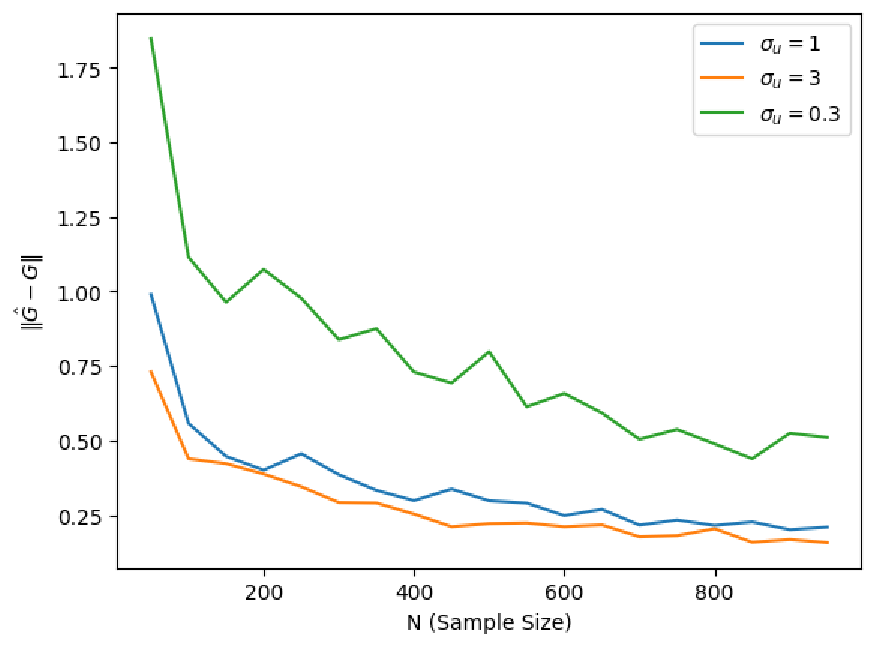
\includegraphics[width=0.8\linewidth]{figure/figure1.pdf}
    \caption{正規分布の分散を変えたときの比較}
    \label{sigma_change}
\end{figure}

図\ref{sigma_change}は,補題\ref{sub_input_alg}を用いる際に,正規分布に従う入力を選択した場合における分散の違いが推定精度に与える影響を比較したものである.


この図から,推定精度は分散の大きさ依存していることが分かる.
入力の制約は,
\begin{equation*}
|u_{t}| \leq 1, \quad \quad  t = 1, 2, \ldots,\bar{N}
\end{equation*}
とした.そのため
正規分布$\mathcal{N}(0, \sigma_u^2)$に従う確率変数$X$ついて,$X>1$のとき$X = 1$,$X<-1$のとき$X = -1$としている.
この分布を丸めた正規分布と呼ぶ.

図\ref{t_vs_c}では,$\mathcal{N}(0, 1)$を丸めた正規分布(clipped normal distribution)と切断正規分布(truncated normal distribution)を比較している.
切断正規分布とは,通常の正規分布を$-a \leq x \leq b$の範囲に制限した分布である.確率密度関数は
\begin{equation*}
f(x|\mu, \sigma, a, b) =
\begin{cases}
0, & \text{if } x \leq a, \\
\frac{\phi(\frac{x-\mu}{\sigma})}{\Phi(\frac{b-\mu}{\sigma}) - \Phi(\frac{a-\mu}{\sigma})}, & \text{if } a < x < b, \\
0, & \text{if } b \leq x.
\end{cases}
\end{equation*}
と表される.ここで$\phi(z), \Phi(z)$はそれぞれ標準正規分布$\mathcal{N}(0, 1)$の確率密度関数,累積分布関数を表しており,
\begin{align*}
    \phi(z) = \frac{1}{\sqrt{2\pi}}e^{-\frac{z^2}{2}}, \quad
    \Phi(z) = \int_{-\infty}^{z} \phi(t) \, dt
\end{align*}
である.
\begin{figure}[htbp]
    \centering
    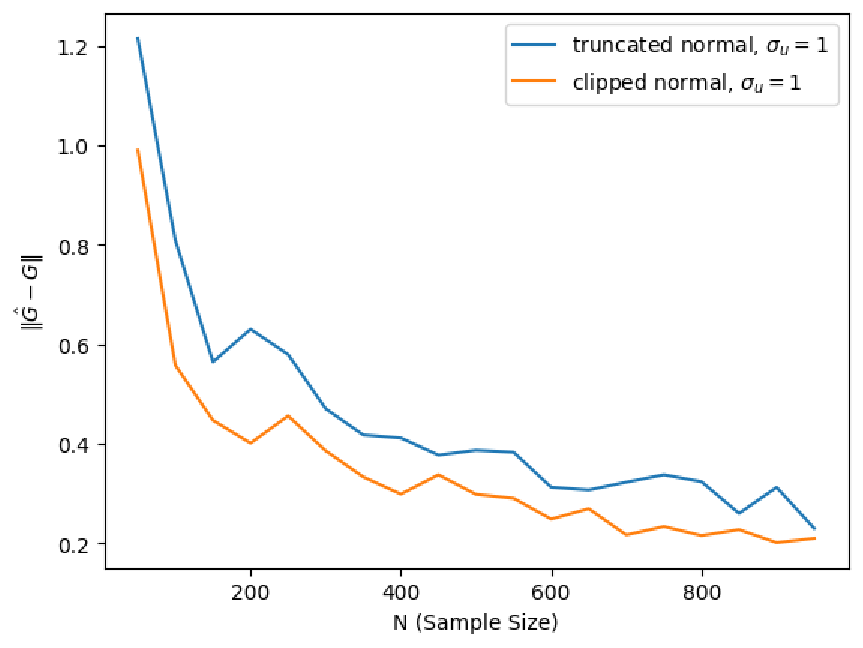
\includegraphics[width=0.8\linewidth]{figure/figure2.pdf}
    \caption{切断正規分布と丸めた正規分布の比較}
    \label{t_vs_c}
\end{figure}
図\ref{t_vs_c}において,切断正規分布は$\mathcal{N}(0, 1)$を$[-1, 1]$で制限している.
丸めた正規分布と切断正規分布を比較すると,丸めた正規分布の方が推定精度が高いことがわかる.

図\ref{u_vs_n_vs_b}では,$\mathcal{N}(0, 1)$を丸めた正規分布と一様分布$\mathcal{U}[-1, 1]$,$\{-1, +1\}$を等確率でとるベルヌーイ試行の3つの分布について比較している.
\begin{figure}[htbp]
    \centering
    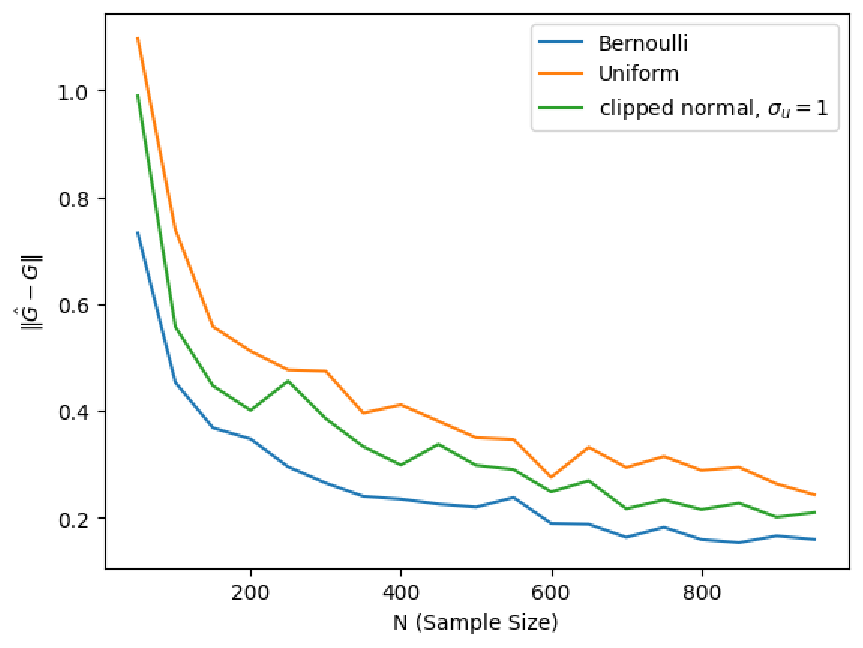
\includegraphics[width=0.8\linewidth]{figure/figure3.pdf}
    \caption{一様分布,ベルヌーイ分布,正規分布の比較}
    \label{u_vs_n_vs_b}
\end{figure}

次の図\ref{x^n}では,
\begin{equation*}
    y = \frac{2k+1}{2}x^{2k}, \quad (-1 \leq x\leq 1)
\end{equation*}
の確率分布と,ベルヌーイ試行について推定誤差を比較している.この分布は$k \to \infty$で$\{-1,+1\}$を等確率でとるベルヌーイ試行に収束する.
$k = 1, 2$の場合である
$f(x) = \frac{3}{2}x^2, f(x) = \frac{5}{2}x^4$と$\{-1, +1\}$を等確率でとるベルヌーイ試行を比較した.

\begin{figure}[htbp]
    \centering
    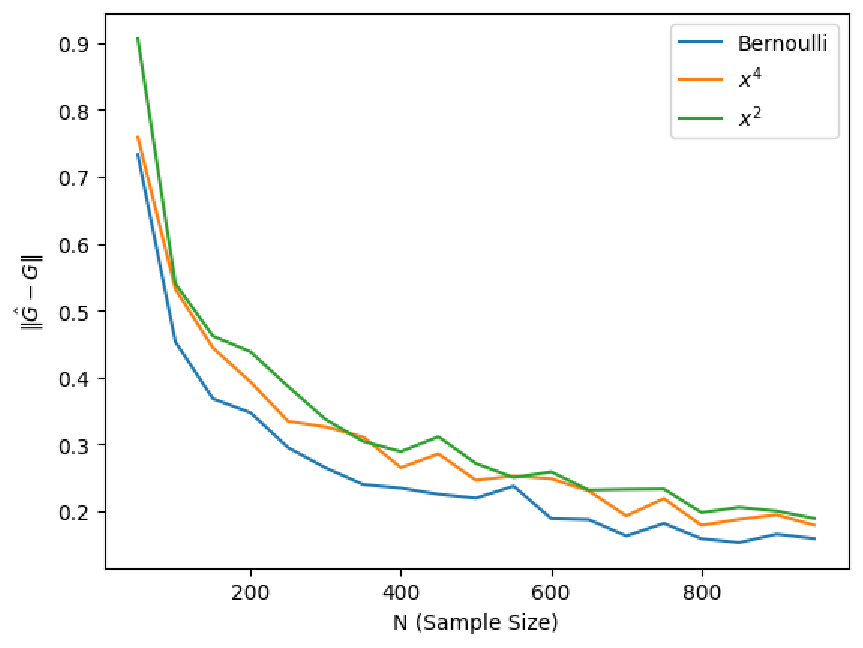
\includegraphics[width=0.8\linewidth]{figure/figure4.pdf}
    \caption{$f(x) = \frac{3}{2}x^2, f(x) = \frac{5}{2}x^4$, ベルヌーイ分布の比較}
    \label{x^n}
\end{figure}

以上の比較から,$\{-1, +1\}$に近い値を高確率でとる分布が推定誤差を小さくしていることがわかる.
\\
実際に$T, N$を固定した低次元の場合について,問題1を解いた場合の結果を以下に示す.
入力の次元は,$p=1$として,各時刻の入力に対し,$|u_t| \leq 1,  (t = 1, 2, \ldots , \bar{N})$とした.
$T = 4, \bar{N} = 7$の場合について,問題1の最適解の1つは,
\begin{equation*}
    U = 
    \begin{bmatrix}
    1 & 1 & -1 & 1 \\
    -1 & 1 & 1 & -1 \\
    1 & 1 & 1 & 1 \\
    1 & -1 & 1 & 1
    \end{bmatrix}
\end{equation*}
であり,最適値は$\sigma_{\text{min}}(U) = 2$である.

また,$T = 4, \bar{N} = 8$の場合について,問題1の最適解の1つは,
\begin{equation*}
    U = 
    \begin{bmatrix}
    1 & 1 & -1 & 1  \\
    1 & 1 & 1 & -1 \\
    1 & 1 & 1 & 1  \\
    -1 & 1 & 1 & 1 \\
    1 & -1 & 1 & 1
    \end{bmatrix}
\end{equation*}
であり,最適値は$\sigma_{\text{min}}(U) = 2$である.
この結果からも$\{-1, +1\}$を等確率でとる分布を選択するのが良いことが分かる.\\

実際に,補題\ref{sub_input_alg}のアルゴリズムに対して,$\{-1, +1\}$を等確率でとる確率変数を用いて入力を設計し,その入力に基づいて得られた最小二乗推定値と,先行研究の入力が正規分布に従い生成される場合の最小二乗推定値を比較した.
用いたサンプル数は,$N = 100$で,$\epsilon = \delta = 0.0001$としたときに補題\ref{sub_input_alg}を満たす$M$として,$M = 100000$とした.表~\ref{table_1}から,入力に制約のない場合よりも推定精度が高いことがわかる.

\begin{table}[h!]
\caption{入力をマルコフパラメータの最小二乗推定値}
\centering
\begin{tabular}{l|rrrr}
                    & $D$      & $CB$     & $CAB$  & $CA^2B$     \\ \hline \hline 
真値                 & 1      & 2      & 1.3 & 0.86 \\ \hline
$\mathcal{N}(0, 1)$ & 1.0923 & 2.0340 & 1.4414  & 0.9217 \\ \hline
提案手法              & 1.0443 & 2.0321 & 1.3640  & 0.8664                   
\end{tabular}
\label{table_1}
\end{table}

\section{推定誤差の上界}
入力を設計した場合の行列$G$の最小二乗推定値と真値の誤差のスペクトルノルムの上界について,以下の定理を示す.

\begin{thm}
$\bar{N} = N + T - 1 $時間の入出力データが与えられたとき,任意の$\delta \in (0, 1)$について$G$の最小二乗推定値$\hat{G}$について,$1- 3\delta$以上の確率で
\begin{align}
\label{upper_bound}
    \|\hat{G}-G\| &\leq \frac{R_w\|F\| +R_e + R_z}{\sigma_{\mathrm{min}}(U)}
\end{align}
が成立する.ただし,
\begin{align*}
    R_w &= \sigma_w\sqrt{ 2\max\{N, pT\}\log{\left(\frac{N+pT}{\delta}\right)}}
    \\
    R_e &=\|C\|\eta^{T-1} \sum_{t = T}^{\bar{N}}\sum_{i = 1}^{t-T-i}\eta^{t-T-i}\|Bu_i\| \\ 
    &\quad + N\frac{\sigma_w\eta^{T-1}}{\sqrt{1-\eta^2}} \|C\| \sqrt{m + \sqrt{8m\log{(2/\delta)}}}
    \\
    R_z &= \sigma_z(\sqrt{N} + \sqrt{m}+ \sqrt{\log{1/\delta}})
\end{align*}
である.
\end{thm}

\begin{proof}
% \textbf{証明: }
まず,ノイズの項$\|Z\|$の上界を与える.
付録Aの補題\ref{Z_bound}より,$1-\delta$以上の確率で
\begin{equation*}
    \|Z\| \leq \sigma_z(\sqrt{N} + \sqrt{m} + \sqrt{\log{1/  \delta}} )
\end{equation*}
が成り立つ.

次に,$\|W\|$の上界を与える.まず,$w_t$がスカラーである場合$(p = 1)$を考える.
\begin{align*}
    W^* &= 
    \begin{bmatrix}
        W_T     & W_{T+1} & \cdots & W_{\bar{N}} \\
        W_{T-1} & W_T     & \cdots & W_{\bar{N}-1} \\
        \vdots  & \vdots  & \ddots & \cdots \\
        W_1     & W_2     & \cdots & W_N
    \end{bmatrix}\in\mathbb{R}^{T \times N} 
\end{align*}
であるから,
\begin{align*}
    B_1 = 
    \begin{bmatrix}
        0 & 0 &\cdots & 0 \\
        0 & 0 &\cdots & 0 \\
        \vdots & \vdots & \ddots &\vdots\\
        1 & 0 & \cdots & 0
    \end{bmatrix}
    , B_2 = 
    \begin{bmatrix}
        0 & 0 &\cdots & 0 \\
        \vdots & \vdots &\ddots & 0 \\
        1 & 0 & \ddots &\vdots\\
        0 & 1 & \cdots & 0
    \end{bmatrix}, \cdots, B_{\bar{N}} = 
    \begin{bmatrix}
        0 & 0 &\cdots & 1 \\
        0 & 0 &\cdots & 0 \\
        \vdots & \vdots & \ddots &\vdots\\
        0 & 0 & \cdots & 0   
    \end{bmatrix}
\end{align*}
と定義すると,
\begin{align*}
    W^* = w_1B_1 + w_2B_2 + \cdots + w_{\bar{N}}B_{\bar{N}} 
\end{align*}
と表すことができる.ここで,
補題\ref{W_bound}から,Wの分散に関する統計量$v(W)$を,
\begin{align*}
    v(W) &= \sigma_w^2\max \left\{ \sum_{k}B_kB_k^*, \sum_{k}B_k^*B_k \right\} \\
    &=\sigma_w^2 \max\{NI, TI\} \\
    &=\sigma_w^2 \max\{N, T\}
\end{align*}
とする.
$w_t \sim \mathcal{N}(0, \sigma_w^2I)$であるから,$w_t$がベクトル$(p >1)$の場合も同様に考えることができ,このとき
$v(W) = \sigma_w^2 \max\{N, pT\}$であるから,
\begin{equation*}
    \mathbb{P}\{ \|W\| \geq t\} \leq \exp{\left(\frac{-t^2}{2\sigma_w^2 \max\{N, pT\}}\right)} 
\end{equation*}
$\exp{\left(\frac{-t^2}{2\sigma_w^2 \max\{N, pT\}}\right)}=\delta$とおき,$\delta$について解くと,
\begin{equation*}
\label{W}
    \mathbb{P} \left\{ \|W\| \leq \sigma_w\sqrt{ 2\max\{N, pT\}\log{\left(\frac{N+pT}{\delta}\right)} }\right\} \geq 1-\delta
\end{equation*}
が成り立つ.

次に,$\|E\|$の項の上界について考える.
\begin{align*}
    e_t &= CA^{T-1}x_{t-T+1} \\
    &= CA^{T-1} 
    \begin{bmatrix}
        B & AB & \ldots & A^{t-T-1}B
    \end{bmatrix}
    \begin{bmatrix}
        u_{t-T}\\
        \vdots\\
        u_1
    \end{bmatrix}\\
    &\quad+ CA^{T-1}
        \begin{bmatrix}
        I & A & \ldots & A^{t-T-1}
    \end{bmatrix}
    \begin{bmatrix}
        w_{t-T}\\
        \vdots\\
        w_1
    \end{bmatrix}
\end{align*}
と展開できる.

\begin{equation*}
    W_t = CA^{T-1} \sum_{i = 0}^{t-T-1}A^iw_{t-T-i}
\end{equation*}
とすると,$e_t$の共分散行列は$\mathbb{E}[W_tW_t^*]$で表されるので,$w_t \sim \mathcal{N}(0, \sigma_w^2I)$であることから,
\begin{align*}
    X_t &= CA^{T-1} \sum_{i = 1}^{t-T} A^{t-T-i}Bu_i\\
    \Sigma(e_t) &=\mathbb{E}[W_tW_t^*] \\
    &= CA^{T-1} \left\{ \sum_{i = 0}^{t-T-1} \sigma_w^2 A^i(A^*)^i \right\}(A^{T-1})^*C^*
\end{align*}
とすると,$e_t$は,$\mathcal{N}(X_t, \Sigma(e_t))$に従う.
また
$\rho(A) \leq \eta$
であるから,
\begin{align*}
    \Sigma(e_t) &\leq CA^{T-1} \left\{ \sum_{i = 0}^\infty \sigma_w^2 A^i(A^*)^i \right\}({A^{T-1}})^*C^*\\
    &\leq \frac{\sigma_w^2\eta^{2(T-1)}}{1-\eta^2}CC^*\\
    & = \Sigma_e
\end{align*}
とすると上界を導出するにあたって,
$e_t \sim \mathcal{N}(X_t, \Sigma_e)$
と見積もってもよい.したがって,
$\tilde{e}_t = (\Sigma_e)^{-1/2}(e_t-X_t)$
は
$\mathcal{N}(0, I_n)$
に従う.これを$e_t$について解くと,
$e_t = (\Sigma_e)^{1/2}(\tilde{e_t})+X_t$
となるので,
\begin{align*}
    \|e_t\| &= \| (\Sigma_e)^{1/2}  \tilde{e}_t  + X_t\| \\
    &\leq \| \Sigma_e \|^{1/2} \| \tilde{e}_t \| + \|X_t\|
\end{align*}
が成り立つ.したがって,\eqref{E}式より,
\begin{align*}
    \|E\| &\leq \|e_T\| + \|e_{T+1}\| + \cdots + \|e_{\bar{N}}\| \\
    &\leq N \| \Sigma_e \|^{1/2} \| \tilde{e}_t \|  +\sum_{t = T}^{\bar{N}}\|X_t\| 
\end{align*}
が成り立つ.ここで,
\begin{align*}
    \sum_{t = T}^{\bar{N}}\|X_t\| &= \sum_{t = T}^{\bar{N}}\|CA^{T-1} \sum_{i = 1}^{t-T}A^{t-T-i}Bu_i\| \\
    &\leq \|C\|\eta^{T-1} \sum_{t = T}^{\bar{N}}\sum_{i = 1}^{t-T}\eta^{t-T-i}\|Bu_i\|
\end{align*}
である.

また,$\|\tilde{e}_t\|^2$は自由度$m$の$\chi$二乗分布に従うので,付録Aの補題\ref{chi^2_bound}より,
\begin{align*}
    \mathbb{P}\left[\left|\frac{1}{m}\|\tilde{e}_t\|^2 -1 \right| \geq t \right] \leq 2e^{-nt^2/8}
\end{align*}
が成り立つ.右辺を$\delta$として整理すると,
$1-\delta$以上の確率で
\begin{equation*}
    \|\tilde{e}_t\| \leq \sqrt{m + \sqrt{8m\log{(2/\delta)}}}
\end{equation*}
が成り立つことが分かる.

以上を組み合わせると$G$の推定誤差の上界\eqref{upper_bound}式が得られる.
\end{proof}

また,今回の問題設定では入力の大きさに上界$|u_{tk}| \leq a,  \quad (\forall t = 1, 2, \ldots,\quad  k = 1, 2, \ldots,p)$を課している.付録Bから,上界,下界のある確率分布から入力を設計しているため,設計した入力はsub-Gaussian性を持つことが分かる.
2章で紹介した定理\ref{thm_prev_error_bound}は,入力がsub-Gaussian性を持つ確率分布から生成されていれば用いることができる.

正規分布$\mathcal{N}(\mu, \sigma^2)$はに従う変数$X$は,パラメータ$\sigma$のsub-Gaussianである.
また,補題\ref{sub_input_alg}を用いて入力を設計する際に選択した$\{-a, +a\}$を等確率でとる確率分布から生成される確率変数も,例\ref{rad_ex}から,パラメータ$a$のsub-Gaussianであることが分かる.したがって,定理\ref{thm_prev_error_bound}や,補題\ref{sub_estimate_y}において入力の分散である$\sigma_u$をsub-Gaussianのパラメータに置き換えて考えることができる.十分大きな$N$における推定誤差の上界について,以下の定理を示す.

\begin{thm}
% \cite[Theorem3.2]{RHKB}
% \cite{RHKB}
\label{thm_prev_error_bound_2}
    $c, C >0$は十分大きな定数である.
    $\rho(A) < 1$であり,$\frac{N}{\log^2{(Np)}} \geq cpT\log^2{(pT)}$であるとする.
    $q = p+n$,$N_w = cTq\log^2{Tq}\log^2{Nq}$とする.
    また,入力がパラメータ$\sigma$の$\mathrm{sub-Gaussian}$である確率変数に従い生成されるとする.
    このとき,高い確率でマルコフパラメータ行列$G$の最小二乗推定値$\hat{G}$について,
    \begin{equation*}
        \| \hat{G}-G \| \leq \frac{R_w\|F\| + R_z + R_e}{\sigma\sqrt{N}}
    \end{equation*}
    が成り立つ.ここで,
    \begin{align*}
        R_z &= 8\sigma_z \sqrt{Tp + m} \\
        R_w &= \sigma_w (\sqrt{N_w} + N_w/\sqrt{N}) \\
        R_e &= C\sigma_e \sqrt{ \left( 1+\frac{mT}{N(1-\rho(A)^{T/2})}  \right)(Tp + m) }
    \end{align*}
    である.また,
    \begin{align*}
        \Phi(A) &= \sup_{\tau \geq 0} \frac{\|A^{\tau}\|}{\rho(A)^{\tau/2}} \\
        \Gamma_{\infty} &= \sum_{i = 0}^{\infty} \sigma_w^2A^i(A^*)^i + \sigma^2  A^iBB^*(A^*)^i
    \end{align*}
    とすると,
    \begin{equation*}
        \sigma_e = \Phi(A)\|CA^{T-1}\|\sqrt{\frac{T\|\Gamma_{\infty}\|}{1-\rho(A)^T}}
    \end{equation*}
    である.
\end{thm}

\chapter{結論}

線形時不変システム同定の有限時間での解析においては,様々な観点から研究が行われている.本研究では,特に部分観測の線形時不変システムにおけるマルコフパラメータの推定に焦点を当てた.従来の研究では,入力信号が正規分布に従い生成されるという理想的な前提のもとで設計されていた.しかし,実際の応用環境では,アクチュエータの出力制約などにより,入力信号に様々な制約が課されることが一般的である.

そこで本研究では,より現実的な問題設定として,アクチュエータの物理的制約により入力信号の大きさに上限がある状況下で,システムの入出力関係を示すマルコフパラメータを推定する手法を提案し,その有効性を数値実験により検証した.具体的には,補題\ref{sub_input_alg}のアルゴリズムを用いる際に,異なる確率分布を用いて入力を設計し,推定誤差を比較した.その結果,一様分布や正規分布と比較して,分散の大きい丸めた正規分布や$\{−1, +1\}$を等確率でとるベルヌーイ試行など,上限値に高確率で近づく確率分布を用いることで,推定精度が向上することが明らかになった.また,推定するマルコフパラメータの数や用いる入出力データセットの数が少ない場合においても,問題1を解いた結果から,ベルヌーイ試行を用いた入力設計が有効であることが確認された.さらに,設計した入力を用いてマルコフパラメータの最小二乗推定を行った際の推定誤差のノルムについて,その理論的な誤差上界を導出した.これにより,制約のある環境下でも適切な入力設計を行うことで推定精度が保証されることを数理的に示した.

今後の課題として,同じ問題設定のもとでより厳密な推定誤差の上界を導出することが挙げられる.また,本研究ではアクチュエータの物理的制約に基づいた入力設計を行ったが,今後は電力消費が制約されるデバイスにおけるエネルギー制約を考慮した入力設計へと発展させることが求められる.さらに,実際の計測環境ではノイズが理想的な正規分布に従わない場合があるため,より現実的なノイズモデルを考慮した解析も重要な課題である.

\chapter*{謝辞}
\addcontentsline{toc}{chapter}{謝辞}
本研究は,著者が大阪大学工学部応用自然科学科応用物理学科目在学中に
大阪大学大学院情報科学研究科情報数理学専攻計画数理学講座において行われたものである.
末筆ながら,本研究を進めるにあたり,御多忙の中,細部にいたるまで御指導と御助言を賜りました
本学准教授 和田孝之先生には深く感謝の意を表すと共に,
厚く御礼を申し上げます.
また,研究を行う上で,終始適切な御助言と御助力を賜りました本学教授 藤崎泰正先生,
事務補佐員 桑原奈美氏には厚く御礼申し上げます.
最後に,貴重な御意見を賜りました計画数理学講座内諸氏に御礼申し上げます.
%

% \bibliography{ref} 
% \bibliographystyle{junsrt}

\begin{thebibliography}{9}

\bibitem{SSSS}
足立: 
システム同定の基礎, 東京電機大学出版局 (2009)

\bibitem{SITF}
L.~Ljung:
\textit{System Identification Theory for the User},
Prentice-Hall, inc. (1999)

\bibitem{HDPA}
R.~Vershynin:
\textit{High-Dimensional Probability An Introduction with Applications in Data Science}, 
Cambridge University Press (2018)

\bibitem{HDSA}
M.~J.~Wainwright:
\textit{High-Dimensional Statistics: A Non-asymptotic Viewpoint}, 
Cambridge University Press (2019)

\bibitem{TEOS}
T.~Hastie, R.~Tibshirani, and J.~Friedman: 
\textit{The Elements of Statistical Learning},
Springer New York (2009)

\bibitem{SLTF}
T.~Anastasios, Z.~Ingvar, M.~Nikolai, and G.~J.~Pappas:
Statistical Learning Theory for Control: A Finite-Sample Perspective,
\textit{IEEE Control Systems Magazine}
\textbf{43}-6, 67/97 (2023)

\bibitem{FTIIU}
M.~K.~S.~Faradonbeh, A.~Tewari, and G.~Michailidis: 
Finite time identification in unstable linear systems, 
\textit{Automatica}, 
\textbf{96}, 342/353 (2018)

\bibitem{FTIOL}
Y.~Jedra and A.~Proutiere: 
Finite-Time Identification of Linear Systems: Fundamental Limits and Optimal Algorithms, 
\textit{IEEE Transactions on Automatic Control}, 
\textbf{68}-5, 2805/2820 (2023)

\bibitem{OTSCO}
S.~Dean, H.~Mania, N.~Matni, B.~Recht, and S.~Tu: 
On the Sample Complexity of the Linear Quadratic Regulator, 
\textit{Foundations of Computational Mathematics}, 
\textbf{20}, 633/679 (2020)

\bibitem{RHKB}
S.~Oymak and N.~Ozay: 
Revising Ho-Kalman-based System Identification: Robustness and Finite-Sample Analysis, 
\textit{IEEE Transactions on Automatic Control}, 
\textbf{67}-4, 1914/1928 (2022)

\bibitem{NAIOL}
Y.~Zheng and N.~Li: 
Non-Asymptotic Identification of Linear Dynamical Systems Using Multiple Trajectories
\textit{IEEE Control Systems Letters}, 
\textbf{5}-5, 1683/1698 (2021)

\bibitem{RAFA}
R.~Tempo, G.~Calafiore, and F.~Dabbene:
\textit{Randomized Algorithms for Analysis and Control of Uncertain Systems}, 
Springer London (2005)

\bibitem{ITTN}
R.~Vershynin:
\textit{Introduction to the non-asymptotic analysis of random matrices}, 
Cambridge University Press (2012)

\bibitem{AITM}
J.~A.~Tropp:
\textit{An Introduction to Matrix Concentration Inequalitues},
Foundations and Trends in Machine Learning 
% \textbf{8}-6, 1/230 
(2015)

\bibitem{IAJI}
D.~J.~H.~Garling:
\textit{Inequalities: A journey into Linear Analysis},
Cambridge University Press (2010)

\end{thebibliography}

\clearpage

\appendix
\chapter{定理1の証明に用いる補題}

\begin{sub}
\label{Z_bound}
% \cite[Corollary5.35]{ITTN}
\cite{ITTN}
$Z$を各要素が$\mathcal{N}(0, \sigma_z^2)$に従う$N \times m$の行列とする.このとき,任意の$\delta \in(0, 1)$について$1-\delta$以上の確率で
\begin{equation*}
    \|Z\| \leq \sigma_z(\sqrt{N} + \sqrt{m} + \sqrt{\log{1/  \delta}} )
\end{equation*}
が成り立つ.
\end{sub}

\begin{sub}
\label{W_bound}
% \cite[Lemma7.7]{AITM}
\cite{AITM}
各行列の次元が$d_1 \times d_2$である複素行列の$n$個の有限列$\{B_k\}, k=1, 2, \ldots, n$を考える.
また$\{\gamma_k\}$を標準正規分布に従う有限列であるとする.
このとき,$Z = \sum_k \gamma_k B_k$とする.
$Z$の分散に関する統計量を
\begin{align*}
    v(Z) &= \max \{ \|\mathbb{E}(ZZ^*)\| , \| \mathbb{E}(ZZ^*) \|\} \\
    &= \max \{ \| \sum_{k=1}^{n} B_kB_k^* \| , \| \sum_{k=1}^{n} B_kB_k^* \|\}
\end{align*}
とする.このとき,任意の$t \geq 0$について,
\begin{equation*}
    \mathbb{P}\{ \|Z\| \geq t\} \leq \left(d_1 + d_2 \exp{\left( \frac{-t^2}{2v(z)} \right)} \right)
\end{equation*}
が成り立つ.
\end{sub}

\begin{sub}
\label{chi^2_bound}
% \cite[Example2.11]{HDSA}
\cite{HDSA}
$z_k \sim \mathcal{N}(0, 1)$に従う独立な変数であるとき,$Y = \sum_{k=1}^{n}z_k^2$は自由度$n$の$\chi$二乗分布に従う.このとき,
\begin{equation*}
    \mathbb{P}\left[\left|\frac{Y}{n} -1 \right| \geq t \right] \leq 2e^{-nt^2/8}
\end{equation*}
が成り立つ.
\end{sub}

\chapter{Sub-Gaussian性をもつ確率変数の性質}
% 以下の内容は文献\cite{HDSA}を参照した.
ここでは本論文で用いるSub-Gaussianの基本的性質をまとめる.

\begin{deff}
    平均が$\mathbb{E}[X] = \mu$である確率変数$X$は,ある正の数$\sigma$が存在し,任意の$\lambda\in \mathbb{R}$について,
    \begin{equation*}
        \mathbb{E}[e^{\lambda(X-\mu)}] \leq e^{\frac{\sigma^2 \lambda^2}{2}}
    \end{equation*}
    が成り立つとき,$X$はパラメータ$\sigma$の$\mathrm{sub-Gaussian}$であるという.
\end{deff}


\begin{ex}
\label{rad_ex}
$\{-a, +a\}$を等確率でとる確率変数を$\epsilon$とする.このとき,
\begin{align}
    \mathbb{E}[e^{\lambda\epsilon}] &= \frac{1}{2}\{e^{-a\lambda} + e^{a\lambda}\} \notag \\
    &=\frac{1}{2} \left\{ \sum_{k = 0}^{\infty}\frac{(-a\lambda)^k}{k!} + \sum_{k = 0}^{\infty}\frac{(a\lambda)^k}{k!} \right\} \notag \\
    &= \sum_{k = 0}^{\infty}\frac{(a\lambda)^{2k}}{(2k)!} \notag \\
    \label{rademacher}
    &\leq e^{a^2\lambda^2/2}
\end{align}
であるから,確率変数$\epsilon$はパラメータ$a$の$\mathrm{sub-Gaussian}$である.
\end{ex}

\begin{ex}
一般に,有界区間$[a, b]$にのみ値をとる$\mathbb{E}[X] = 0$である確率変数$X$について,$X'$を$X$と同じ分布に従う独立な別の確率変数であるとする.
$\mathbb{E}[X'] = 0$,凸関数$f(x) = e^x$に対して,$\mathrm{Jensen}$の不等式$(f(\mathbb{E}[X]) \leq \mathbb{E}[f(X)])$\cite{IAJI}を適用すると,
\begin{equation*}
    \mathbb{E}[e^{\lambda X}] = \mathbb{E}_X[e^{\lambda(X-\mathbb{E}_{X'}[X'])}] \leq \mathbb{E}_{X, X'}[e^{\lambda (X-X')}]
\end{equation*}
が成り立つ.さらに,$\{-1, +1\}$を等確率でとる確率変数を$\epsilon$として導入すると,
\begin{align*}
    \mathbb{E}_{\epsilon}[e^{\lambda \epsilon (X-X')}] &= \frac{1}{2}e^{\lambda(X-X')}+\frac{1}{2}e^{-\lambda(X-X')} \\
    &= e^{\lambda (X-X')} 
\end{align*}
が成り立つ.
$X, X'$は,同じ分布に従う独立な変数であるため,$X-X'$, $X'-X$を新たな確率変数と置くと同じ分布に従うからである.また,\eqref{rademacher}式において,$\lambda \to \lambda(X-X')$とすると
\begin{equation*}
    \mathbb{E}_{\epsilon}[e^{\lambda \epsilon (X-X')}] \leq \mathbb{E}_{X, X'}[e^{\lambda^2 (X-X')^2/2}]
\end{equation*}
が成り立つ.$X, X'\in [a, b]$であるから,$|X-X'|\leq |b-a|$であるので,.
\begin{align*}
    \mathbb{E}[e^{\lambda X}] &\leq \mathbb{E}_{X, X'}[e^{\lambda^2 (X-X')^2/2}] \\
    &\leq e^{\lambda^2 (b-a)^2/2}
\end{align*}
が成り立つ.
したがって,$X$は少なくともパラメータ$b-a$の$\mathrm{sub-Gaussian}$である.
\end{ex}

sub-Gaussian性は,正規分布と同様の集中不等式を適用できるため期待値周辺の集中性やサンプル数と精度の関係を評価する際に広く利用される.






\end{document}
}